\documentclass[conference]{IEEEtran}
\IEEEoverridecommandlockouts
% The preceding line is only needed to identify funding in the first footnote. If that is unneeded, please comment it out.

\usepackage{cite}
\usepackage{amsmath,amssymb,amsfonts}
\usepackage{algorithmic}
\usepackage[printonlyused]{acronym}
\usepackage{graphicx}
\usepackage{textcomp}
%\usepackage[backend=bibtex,style=IEEEtr]{biblatex}


\def\BibTeX{{\rm B\kern-.05em{\sc i\kern-.025em b}\kern-.08em
    T\kern-.1667em\lower.7ex\hbox{E}\kern-.125emX}}
\begin{document}

\title{Activity Recognition with mobile devices\\
}

\author{\IEEEauthorblockN{1\textsuperscript{st} Simon Angerbauer}
\IEEEauthorblockA{\textit{Mobile Computing} \\
\textit{University Of Applied Sciences Upper Austria}\\
Hagenberg, Austria \\
simon.angerbauer@students.fh-hagenberg.at}
\and
\IEEEauthorblockN{2\textsuperscript{nd} Paul Schmutz}
\IEEEauthorblockA{\textit{Mobile Computing} \\
\textit{University Of Applied Sciences Upper Austria}\\
Hagenberg, Austria \\
paul.schmutz@students.fh-hagenberg.at}
\and
\IEEEauthorblockN{3\textsuperscript{rd} Roman Socovka}
\IEEEauthorblockA{\textit{Mobile Computing} \\
\textit{University Of Applied Sciences Upper Austria}\\
Hagenberg, Austria \\
roman.socovka@students.fh-hagenberg.at}
}

\maketitle

\begin{abstract}
This document is a model and instructions for \LaTeX.
This and the IEEEtran.cls file define the components of your paper [title, text, heads, etc.]. *CRITICAL: Do Not Use Symbols, Special Characters, Footnotes, 
or Math in Paper Title or Abstract.
\\
\\
\\
\\
\\
\\
\\
\\
\\
\\
\\
\\
\\
\\
\\
\\
TODO
\end{abstract}

\begin{IEEEkeywords}
Human Activity Recognition, accelerometer, movement pattern detection
\end{IEEEkeywords}

\section{Introduction -- Simon}
asdfas
\\
\\
\\
\\
\\
\\
\\
\\
\\
\\
\\
\\
\\
\\
\\
\\
\\
\\
\\
\\
\\
\\
\\
\\
\\
\\
\\
\\
\\
\\
\\
\\
\\
\\
\\
\\
\\
\\
\\
\\
\\
\\
\\
\\
\\
\\
\\
\\
\\
\\
\\
\\
\\
\\
\\
\\
intro


\section{Related Work -- Paul}
blbla
Refer to articles, how they collected data
did they use mobile phones or separate acceleration sensor devices
body placement of the sensor
significant difference of the results with varying orientation of the phone/sensor. As the performance of algorithms and devices have increased, these problems can be dealt with by now. Also wearing the sensor at different body parts is worsening the situation. Therefore a training phase combined with an AI learning algorithm can help to improve detection results.
Kwapisz2011 ~\cite{Kwapisz2011} however is using orientation of the 3 tri-axial sensor to distinguish between standing and sitting, which is not a real-world scenario for everybody as every individual user might carry the phone in a different way.
results are more precise with multiple sensors, but cell phones are the easiest solution to spread the capability of measuring and classifying movement patterns
real-time processing at low cost ~\cite{Brezmes2009}
The experimental results show that when the sensor is placed on different rigid body, different models are required for certain activities ~\cite{Henpraserttae2011}.
bla
\\
\\
\\
\\
\\
\\
\\
\\
\\
\\
\\
\\
\\
\\
\\
\\
\\
\\
\\
\\
\\
\\
\\
\\
\\
\\
\\
\\
\\
\\
\\
\\
\\
\\
\\
\\
\\
\\
\\
\subsection{Subsection blabla}
subsection
\newpage
\section{Evaluation -- Simon}

\subsection{Results}
\begin{figure}[!htb]
  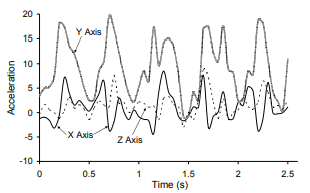
\includegraphics[width=\linewidth]{walking.png}
  \caption{Walking}
  \label{fig:walking}
\end{figure}
\begin{figure}[!htb]
  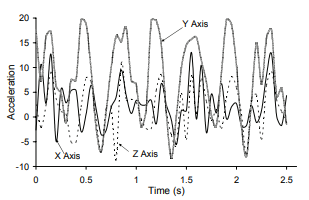
\includegraphics[width=\linewidth]{jogging.png}
  \caption{Jogging}
  \label{fig:jogging}
\end{figure}
\begin{figure}[!htb]
  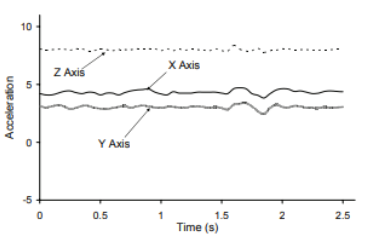
\includegraphics[width=\linewidth]{sitting.png}
  \caption{Sitting}
  \label{fig:sitting}
\end{figure}
\begin{figure}[!htb]
  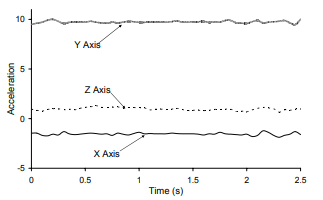
\includegraphics[width=\linewidth]{standing.png}
  \caption{Standing}
  \label{fig:standing}
\end{figure}
\begin{figure}[!htb]
  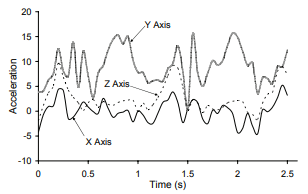
\includegraphics[width=\linewidth]{ascending_stairs.png}
  \caption{Ascending Stairs}
  \label{fig:ascendingStairs}
\end{figure}
\begin{figure}[!htb]
  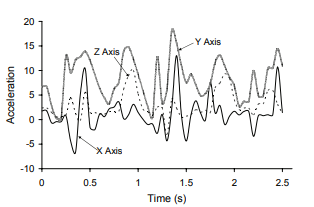
\includegraphics[width=\linewidth]{descending_stairs.png}
  \caption{Descending Stairs}
  \label{fig:descendingStairs}
\end{figure}

\newpage

\subsection{Analysis}

TODO some analysis shit

\section{Conclusion -- Paul}

TODO Conclude or smth

\section*{List of Abbreviations}
\begin{acronym}[XXXXXXXX]
 \acro{HAR}{Human Activity Recognition}
 \acro{AI}{Artificial Intelligence}
\end{acronym}
ias
\\
\\
\\
\\
\\
\\
\\
\\
\\
\\
\\
\\
\\
\\
\\
\\
\\
\\

TODO Abbreviations

\addcontentsline{toc}{section}{References}
\bibliographystyle{unsrt}
\bibliography{references}
asdfiajsd
%%%----------------------------------------------------------
%\MakeBibliography                        				% references
%%%----------------------------------------------------------
%\printbibliography
%\bibliography{references}  	% name of bibliography file (references.bib)
%\bibliographystyle{ieeetr}
\\
\\
\\
\\
\\
\\
\\
\\
\\
\\
\\
\\
\\
\\
\\
\\
\\
\\
\\
\\
\\
\\
\\
\\
TODO Refs



\end{document}
